\documentclass[12pt,fleqn]{article}\usepackage{../common}
\begin{document}
En Yakin k-Komsu (k-Nearest Neighbor)

Yapay Ogrenim alaninda ornek bazli ogrenen algoritmalardan bilinen kNN,
egitim verinin kendisini siniflama (classification) amacli olarak kullanir,
yeni bir model ortaya cikartmaz. Algoritma soyle isler: etiketleri bilinen
egitim verisi alinir ve bir kenarda tutulur. Yeni bir veri noktasi
gorulunce bu veriye geri donulur ve o noktaya ``en yakin'' k tane nokta
bulunur. Daha sonra bu noktalarin etiketlerine bakilir ve cogunlugun
etiketi ne ise, o etiket yeni noktanin etiketi olarak kabul edilir.

``En yakin'' sozu bir kordinat sistemi anlamina geliyor, ve kNN, aynen
k-Means ve diger pek cok kordinatsal ogrenme yontemi gibi eldeki cok
boyutlu veri noktalarinin elemanlarini bir kordinat sistemindeymis gibi
gorur. Kiyasla mesela APriori gibi bir algoritma metin bazli veriyle oldugu
gibi calisabilirdi.

Peki arama baglaminda, bir veri obegi icinden en yakin noktalari bulmanin
en basit yolu nedir? Listeyi bastan sonra taramak (kaba kuvvet yontemi
-brute force-) ve her listedeki nokta ile yeni nokta arasindaki mesafeyi
teker teker hesaplayip en yakin k taneyi icinden secmek bir yontem. Bu
basit algoritmanin yuku $O(N)$'dir. Eger tek bir nokta ariyor olsaydik,
bu kabul edilebilir olabilirdi. Fakat genellikle bir siniflayici
algoritmanin surekli islemesi, mesela bir online site icin gunde
milyonlarca kez bazi kararlari almasi gerekebilir. Bu durumda ve $N$'in cok
buyuk oldugu sartlarda, ustteki hiz bile yeterli olmayabilir.

Arama islemini daha hizli yapmanin yollari var. Akilli arama algoritmalari
kullanarak egitim verilerini bir agac yapisi uzerinden tarayip erisim
hizini $O(\log N)$'e indirmek mumkundur.

K�re Aga�lar� (Ball Tree -BT-) 

Bir noktanin diger noktalara yakin olup olmadiginin hesabinda yapilmasi
gereken en pahali islem nedir? Mesafe hesabidir. BT algoritmasinin puf
noktasi bu hesabi yapmadan, noktalara degil, noktalari kapsayan
``kurelere'' bakarak hiz kazandirmasidir. Noktalarin her biri yerine o
noktalari temsil eden kurenin mihenk noktasina (pivot -bu nokta merkez de
olabilir, herhangi bir baska nokta da-) bakilir, ve oraya olan mesafeye
gore bir kure altindaki noktalara olabilecek en az ve en fazla uzaklik
hemen anlasilmis olur.

Mesela elimizde alttaki gibi noktalar var ve kureyi olusturduk. 

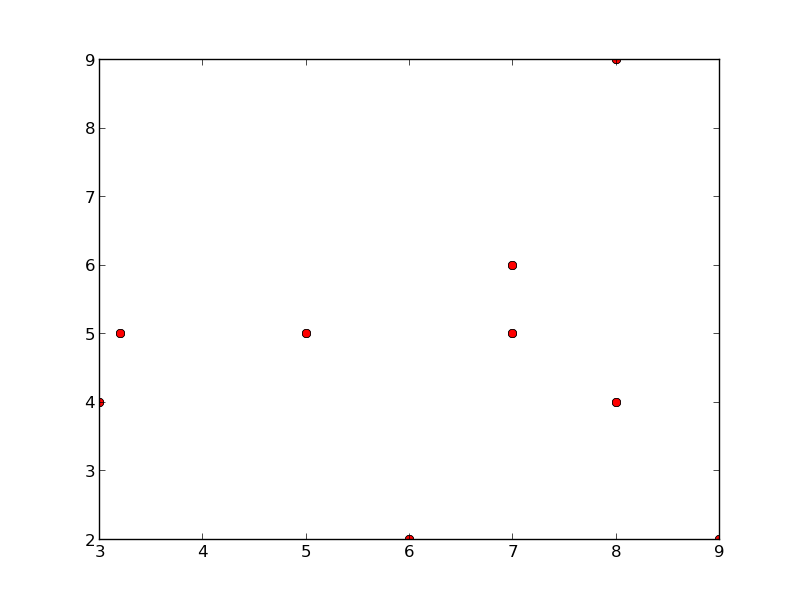
\includegraphics[height=6cm]{knn0.png}

Bu kureyi kullanarak kure disindaki herhangi bir nokta $q$'nun kuredeki
``diger tum noktalar $x$'e'' olabilecegi en az mesafenin ne olacagini
ucgensel esitsizlik ile anlayabiliriz.

Ucgensel esitsizlik 

\[ |x,y| \le |x,z| + |z,y| \]

$||$ operatoru norm operatoru anlamina gelir ve uzaklik hesabinin
genellestirilmis halidir. Konu hakkinda daha fazla detay icin {\em
  Fonksinel Analiz} ders notlarimiza bakabilirsiniz. Kisaca soylenmek
istenen iki nokta arasinda direk gitmek yerine yolu uzatirsak, mesafe
artacagidir. Tabii uzaklik, yol, nokta gibi kavramlar tamamen soyut matematiksel
ortamda da isleyecek sekilde ayarlanmistir. Mesela mesafe (norm) kavramini
degistirebiliriz, Oklitsel yerine Manhattan mesafesi kullaniriz, fakat bu
kavram bir norm oldugu ve belirttigimiz uzayda gecerli oldugu icin ucgensel
esitsizlik uzerine kurulmus tum diger kurallar gecerli olur. 


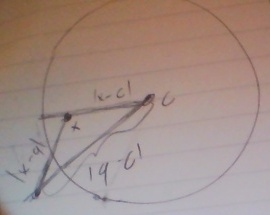
\includegraphics[height=6cm]{tri1.png}

Simdi diyelim ki disaridaki bir $q$ noktasindan bir kure icindeki diger tum
$x$ noktalarina olan mesafe hakkinda bir seyler soylemek istiyoruz. Ustteki
sekilden bir ucgensel esitsizlik cikartabiliriz,

\[ |x-c| + |x-q| \ge |q-c|  \]

Bunun dogru bir ifade oldugunu biliyoruz. Peki simdi yaricapi bu ise dahil
edelim, cunku bu hesap bir kere yapilip kure seviyesinde depolanacak ve bir
daha hesaplanmasi gerekmeyecek, algoritmayi hizlandiracak bir sey olabilir
bu. Eger $|x-c|$ yerine yaricapi kullanirsak, esitsizlik hala gecerli olur,

\[ radius + |x-q| \ge |q-c|  \]

cunku radius $|x-c|$'ten kesinlikle daha buyuktur (Kure Agaclari yaricapi
aynen boyle olmasi icin ayarlayacak). Yaricapi saga gecirelim,

\[ |x-q| \ge |q-c| - radius \]

Boylece guzel bir tanim elde ettik. Yeni noktanin kuredeki herhangi bir
nokta $x$'e olan uzakligi, yeni noktanin mihenke olan uzakliginin yaricapi
cikartilmis halinden {\em muhakkak} fazladir. Yani bu cikartma isleminden
ele gecen rakam yeni noktanin $x$'e uzakligina bir ``alt sinir (lower
bound)'' olarak kabul edilebilir. Diger tum mesafeler bu rakamdan daha
buyuk olacaktir. 

Boylece ne elde ettik? Sadece bir yeni nokta, mihenk ve yaricap kullanarak
kuredeki ``diger tum noktalar hakkinda'' bir irdeleme yapmamiz mumkun
olacak. Bu noktalara teker teker bakmamiz gerekmeyecek. Bunun nasil ise
yaradigini algoritma detaylarinda gorecegiz. 

Benzer sekilde 

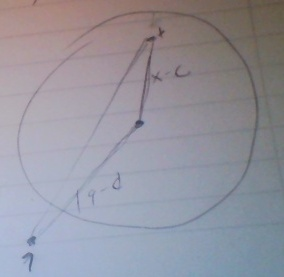
\includegraphics[height=6cm]{tri2.png}

Bu ne diyor? 

\[ |q-c| + |x-c| \ge |q-x| \]

$|x-c|$ yerine yaricap kullanirsak, sol taraf buyuyecegi icin buyukluk hala
buyukluk olarak kalir, 

\[ |q-c| + radius \ge |q-x| \]

ama yine daha genel ve hizli hesaplanan bir kural elde ederiz (onceki
ifadeye benzemesi icin yer degisikligi yapalim

\[ |q-x| \le |q-c| + radius \]

Bu ifade ne diyor? Yeni noktanin mihenke olan uzakligina yaricap
``eklenirse'' bu uzakliktan, buyuklukten daha buyuk bir yeni nokta - kure
 mesafesi olamaz, kuredeki hangi nokta olursa olsun. Bu esitsizlik te bize
 bir ust sinir (upper bound) vermis oldu. 

Algoritma

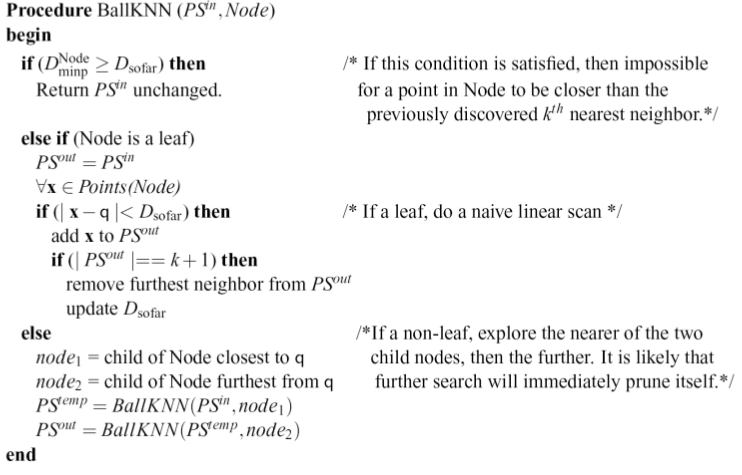
\includegraphics[height=7cm]{alg.png}

Kure Agaclari (BT) metotu once kureleri olusturmalidir. Bu kureler
hiyerarsik sekilde planlanir, tum noktalarin icinde oldugu bir ``en ust
kure'' vardir her kurenin iki tane cocuk kuresi olabilir. Belli bir
(disaridan tanimlanan) minimum $r_{min}$ veri noktasina gelinceye kadar
sadece noktalari kapsayan kureler olusturulur, kureler noktalari
sahiplenmezler. Fakat bu $r_{min}$ sayisina erisince (artik oldukca
alttaki) kurelerin uzerinde noktalar konur. 

Once tek kurenin tanimina bakalim: bir kure tanimi icin eldeki veri icinden
herhangi bir tanesi mihenk olarak kabul edilebilir. Daha sonra bu mihenkten
diger tum noktalara olan uzaklik olculur, ve en fazla, en buyuk olan
uzaklik yaricap olarak kabul edilir (her seyi kapsayabilmesi icin). ``Tum
diger noktalara bakilmasi'' dedik, bundan kacinmaya calismiyor muyduk?
Fakat dikkat, ``kure olusturulmasi'' evresindeyiz, k tane yakin nokta arama
evresinde degiliz. Yapmaya calistigimiz aramalari hizlandirmak - egitim /
kure olusturmasi bir kez yapilacak ve bu egitilmis kureler bir kenarda
tutulacak ve surekli aramalar icin ardi ardina kullanilacaklar. 


\lstinputlisting[language=Python]{dist.py}

\lstinputlisting[language=Python]{knn.py}

Kaynaklar

[1] Liu, Moore, Gray, {\em New Algorithms for Efficient High Dimensional
Non-parametric Classification}



\end{document}
